% Compile with XeLaTeX, TeXLive 2013 or more recent
\documentclass{beamer}

% Base packages
\usepackage{fontspec}

\usepackage{xunicode}
\usepackage{xltxtra}

\usepackage{amsfonts}
\usepackage{amsmath}
\usepackage{longtable}
\usepackage{csquotes}
\usepackage{standalone}

\usepackage{graphicx}
\graphicspath{{./images/}}

\usepackage{tikz}
\usetikzlibrary{arrows,decorations.pathmorphing,backgrounds,positioning,fit,petri}

\usepackage{listings}
\lstset{language=C, basicstyle=\ttfamily, breaklines=true, keepspaces=true, keywordstyle=\color{blue}}

% Setup Russian hyphenation
\usepackage{polyglossia}
\setdefaultlanguage[spelling=modern]{russian} % for polyglossia
\setotherlanguage{english} % for polyglossia

% Setup fonts
\newfontfamily\russianfont{CMU Serif}
\setromanfont{CMU Serif}
\setsansfont{CMU Sans Serif}
\setmonofont{CMU Typewriter Text}

% Be able to insert hyperlinks
\usepackage{hyperref}
\hypersetup{colorlinks=true, linkcolor=black, filecolor=black, citecolor=black, urlcolor=blue , pdfauthor=Grigory Rechistov <grigory.rechistov@phystech.edu> and Evgeny Yulyugin <yulyugin@gmail.com>, pdftitle=Программное моделирование вычислительнызх систем}
% \usepackage{url}

% Misc optional packages
\usepackage{underscore}
\usepackage{amsthm}

% A new command to mark not done places
\newcommand{\todo}[1][]{{\color{red}TODO\ #1}}

\newcommand{\abbr}{\textit{англ.}\ }

\subtitle{Курс «Программное моделирование вычислительных систем»}
\subject{Лекция}
\date{\today}
\pgfdeclareimage[height=0.5cm]{ilab-logo}{../common/ilab-noletters.png}
\logo{\pgfuseimage{ilab-logo}}

\typeout{Copyright 2014 Grigory Rechistov and Evgeny Yulyugin}

\usetheme{Berlin}
\setbeamertemplate{navigation symbols}{}%remove navigation symbols


\title{Языки разработки моделей и аппаратуры}
\author[Григорий Речистов]{Григорий Речистов \\ \small{\href{mailto:grigory.rechistov@phystech.edu}{grigory.rechistov@phystech.edu}}}

\begin{document}

\begin{frame}
\titlepage
\end{frame}

\section*{Обзор}

\begin{frame}{На прошлой лекции}
\begin{itemize}
\item Оптимистичные схемы
\item Откат состояния 
\item Time Warp и virtual time \pause
\item Вопрос: как выполнять вывод (\texttt{printf}) в оптимистичной симуляции?
\end{itemize}

\end{frame}

\begin{frame}{На этой лекции}
\tableofcontents
\end{frame} 

\begin{frame}{Общая схема моделируемой системы}

\centering

\inputpicture{parsim-overview}
    
\end{frame}

% \begin{frame}{Препятствия}
% \begin{enumerate}
% \item    Возможность гонок данных (data race)
% \item    Возможность взаимоблокировок 
% \item    Неэффективная работа параллельного приложения 
% \item    Недетерминистичность
% \end{enumerate}
% \end{frame}

\section{Атомарные инструкции}

\begin{frame}{Атомарные инструкции}

\begin{tikzpicture}[>=latex]

\node[draw, circle] (core1) {Ядро 1};

\node[draw, circle, right = of core1] (core2) {Ядро 2};

\node[draw, circle, right = of core2] (core3) {Ядро 3};

\node[draw, circle, right = of core3] (core4) {Ядро 4};

\node[below = 2cm of core1] (c1) {};
\node[below = 2cm of core4] (c2) {};

\node[draw, fit = (c1) (c2) ] (shmem) {Общая память} ;

\path (core2.south) -- (core3.south) node[midway, yshift = -1cm] (lock) {\texttt{LOCK}};
\draw[thick,] (core2) |- (lock);
\draw[thick,->] (lock) -- (shmem);

\path (core1.south) |- (lock) coordinate[midway] (block1); %{X};
\path (core3.south) |- (lock) coordinate[midway] (block3); %{X};
\path (core4.south) |- (lock) coordinate[midway] (block4); %{X};

\draw[->] (core1.south) -- (block1);
\draw[->] (core3.south) -- (block3);
\draw[->] (core4.south) -- (block4);

\draw[dashed] (block1) -- (lock);
\draw[dashed] (lock)   -- (block3);
\draw[dashed] (block3) -- (block4);

\end{tikzpicture}

\begin{itemize}
    \item {Read--Modify--Write} для ячейки в памяти
    \item Средства реализации семафоров
    \item «Дорогие» для исполнения \pause
    \item {Вопрос}: нужны ли атомарные инструкции для однопроцессорных систем?
\end{itemize}

\end{frame}

\begin{frame}{Симуляция инструкций}

\begin{enumerate}
    \item Использование хозяйских инструкций
    \item Использование критических секций
    \item Использование транзакций
\end{enumerate}
\end{frame}

\begin{frame}{Использование хозяйских инструкций}
\begin{itemize}
    \item Разные ISA для атомарных инструкций (напр. IA-32 --- больше 10 инструкций, ARM --- две)
    \item Не все атомарные операции одинаково \emph{сильны} (consensus number)~\cite{consensus-number}
    \begin{itemize}
        \item $\infty$ --- Mem-Mem, CAS, LL/SC
        \item 2 --- TAS, SWAP, FAA
        \item 1 --- атомарное чтение и запись
    \end{itemize}
    \item Метод наиболее удобен в случаях совпадения архитектур хозяина и гостя
\end{itemize}
\end{frame}

\begin{frame}{Использование критических секций}
\begin{itemize}
    \item Хозяйская критическая секция для моделирования одной атомарной операции \pause \dots{} но это не работает
    \item Пример~\cite{coremu}: взятие семафора с помощью CAS, освобождение --- с помощью атомарной записи
\end{itemize}

\begin{tikzpicture}[font=\footnotesize\ttfamily, inner sep =1pt]
\node    (core1) {\rmfamily Процессор 1};
\node[right = 4cm of core1]  (core2) {\rmfamily Процессор 2};

\node[below = 0.25cm of core1.west, anchor = north west]    (unlock) {sem_unlock:};
\node[below = 0.25cm of core2.west, anchor = north west]    (lock) {sem_lock:};

\node[align=left, below = 0.25cm of lock.west, anchor = north west] (try-part) {try:\\ r10 = 1};
\node[draw=black!30, align=left, below = 0cm of try-part.south west, anchor = north west] (xchg-part) {\textbf{xchg addr, r10}};
\node[align=left, below = 0cm of xchg-part.south west, anchor = north west] (comp-part) {if (r10 == 0 ) \\
       \ \ goto success\\
       fail:\\
       pause\\
       if (*addr != 0)\\
       \ \ goto fail\\
       goto try\\
       success:
};

\node[align=left, left = 1.5cm of xchg-part.west, anchor= south] (xchg-upper) {TO = r10\\ T1 = *addr};
                   
\node[align=left, below = 0cm of xchg-upper.south west, anchor = north west] (xchg-lower)  {*addr = T0\\r10 = T1};

\node[draw, align = left, left= 1.3cm of xchg-lower.north west, anchor = east] (addr-0) {*addr = 0}; 

\node[draw=black!30, fit = (lock) (try-part) (xchg-part) (comp-part)]  {};

\node[draw=black!30, fit = (xchg-upper) (xchg-lower)] (frame1) {};

\node[below = 4cm of core1] (unlock-end) {} ;
\node[draw=black!30, fit = (unlock) (addr-0) (unlock-end)] {} ; 

% add an ugly connector between XCHG and its internals
\path[fill=white, draw=black!30] (frame1.north east) -- (xchg-part.north west) -- (xchg-part.south west) -- (frame1.south east) ;

% finall, a race
\draw[->] (addr-0.east) -- (xchg-lower.north) node[font=\rmfamily\tiny, pos= 0.42, below, text width=1cm] {Гонка данных};

\end{tikzpicture}

\end{frame}

\begin{frame}{Использование транзакций}
    \begin{itemize}
        \item Не предотвращать, а детектировать гонки данных
        \item Повторять попытку атомарной операции в случае неуспеха
        \item Используются хозяйские инструкции CAS или (лучше) LL/SC
    \end{itemize}
\end{frame}

\section{Модели памяти}

\begin{frame}{Консистентность памяти}
\begin{itemize}
    \item Между процессорами и ОЗУ может лежать несколько буферов (кэши, очереди)
    \item Возможны ситуации, в которых разные процессоры «видят» разные значения для одних и тех ячеек
    \item Правила, которые определяют допустимые порядки видимости значений для архитектуры --- модель консистентности памяти \pause
    \item Модели консистентности различаются между собой
\end{itemize}

\end{frame}

\begin{frame}{Отношение строгости}

Из~\cite{consistency-report}

\centering

\begin{tikzpicture}[>=latex, inner sep = 1pt]
    \node at (0,0) (sc) {SC} ;
    \node at (2, -1) (ibm370) {IBM-370};
    \node at (-0.5, -1.5) (tso) {TSO};
    \node at (1, -1.8) (pc) {PC};
    \node at (-0.5, -2.5) (pso) {PSO} ;
    \node at (-2.5, -3) (wo) {WO} ;
    \node at (-.5, -3.5) (rcsc) {RCsc} ;
    \node at (1, -4) (rcpc) {RCpc} ;
    \node at (3, -3) (alpha) {Alpha} ;
    \node at (1.5, -3.5) (rmo) {RMO} ;
    \node at (5, -3.5) (powerpc) {PowerPC} ;
    
    \draw[->] (wo) -- (sc);
    \draw[->] (tso) -- (sc);
    \draw[->] (ibm370) -- (sc);
    \draw[->] (pc) -- (tso);
    \draw[->] (pso) -- (tso);
    \draw[->] (pc) -- (ibm370);
    \draw[->] (rcsc) -- (wo);
    \draw[->] (rcpc) -- (rcsc);
    \draw[->] (rcpc) -- (pc);
    \draw[->] (rmo) -- (alpha);
    \draw[->] (powerpc) -- (alpha);
    \draw[->] (alpha) -- (ibm370);
\end{tikzpicture}
\end{frame}

\begin{frame}{Что же делать? Барьеры памяти}
\begin{itemize}
    \item Устанавливают частичный порядок для операций
    \item Т.е. какие из доступов в каком направлении могут опережать соседние
    \item Чтение, запись, доступ к устройствам, чтение инструкций
    \item Примеры инструкций: \texttt{sfence}, \texttt{lfence}, \texttt{mfence}; \texttt{mf}, \texttt{ld.acq}, \texttt{ld.rel}; \texttt{eioeio}, \texttt{sync}; \texttt{cpuid}
	\item Атомарные инструкции не обязательно являются барьерами!
\end{itemize}
\end{frame}

\begin{frame}{Сравнение архитектур}
Из~\cite{whymb}
\begin{center}
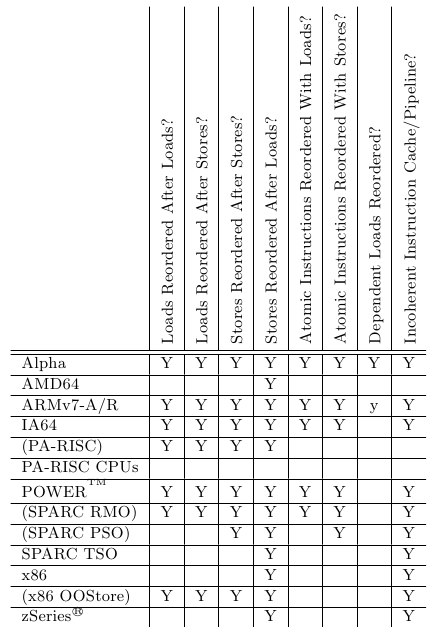
\includegraphics[height=0.8\textheight]{barrier-arch.png}
\end{center}
\end{frame}

\section{Примеры симуляторов}

\begin{frame}{Практические параллельные симуляторы}
\begin{itemize}
    \item Simics
    \item Graphite
    \item SimOS
    \item Coremu
    \item Pqemu
    \item BigSim
    \item DynamoRIO
\end{itemize}
\end{frame}

\begin{frame}{Дополнительные вопросы параллельной симуляции}
\begin{itemize}
    \item Параллельная двоичная трансляция
    \item Распределённая общая память \pause
    \item Почему параллельная симуляция настолько сложна? \pause \textit{<<\dots необходимо определить, может или нет сообщение $E_1$ быть обработано одновременно с $E_2$. Но каким образом узнать, влияет или нет $E_1$ на $E_2$, без его симуляции?>>}
\end{itemize}    
\end{frame}

\section{Литература}

\begin{frame}[allowframebreaks]{Рекомендуемая литература}
\begin{thebibliography}{99}
    \bibitem{consensus-number} \textit{Maurice Herlihy}. “Wait-Free Synchronization” \url{http://cs.brown.edu/~mph/Herlihy91/p124-herlihy.pdf}
    \bibitem{coremu} \textit{Zhaoguo Wang et al.} COREMU: a Scalable and Portable Parallel Full-System Emulator \url{http://ppi.fudan.edu.cn/_media/publications\%3Bcoremu-ppopp11.pdf},
    \bibitem{consistency-report} \textit{Kourosh Gharachorloo} Memory Consistency Models for Shared-Memory Multiprocessors. \url{http://infolab.stanford.edu/pub/cstr/reports/csl/tr/95/685/CSL-TR-95-685.pdf}
    \bibitem{whymb} \textit{Paul E. McKenney} Memory Barriers: a Hardware View for Software Hackers \url{http://citeseerx.ist.psu.edu/viewdoc/summary?doi=10.1.1.152.5245}
%     \bibitem{} Paul E. McKenney. Memory Ordering in Modern Microprocessors
    \bibitem{pqemu} \textit{Jiun-Hung Ding et al.} PQEMU: A Parallel System Emulator Based on QEMU \url{http://dx.doi.org/10.1109/ICPADS.2011.102}
    \bibitem{itanium-mem-order} \textit{Intel Corporation} A Formal Specification of {Intel}® {Itanium}® Processor Family Memory Ordering
\end{thebibliography}
\end{frame}


\section*{Конец}
% The final "thank you" frame 
\begin{frame}

{\huge{Спасибо за внимание!}\par}

\vfill

Материалы курса выкладываются на сайте \url{http://iscalare.mipt.ru/material/course_materials/}

\vfill

\tiny{\textit{Замечание}: все торговые марки и логотипы, использованные в данном материале, являются собственностью их владельцев. Представленная здесь точка зрения отражает личное мнение автора, не выступающего от лица какой-либо организации.}

\end{frame}

% \section{Резерв}

\end{document}
